\chapter{Optimization Using Mathematical Programs with Complementarity Constraints} \label{cap:mpcc}

\section{Formulation of Interconnected Power and Gas Systems} \label{sec:formulation}


An interconnected system can be effectively represented by a directed graph denoted as $\left\lbrace\mathcal{N}, \mathcal{E}\right\rbrace$, where the sets of units $\mathcal{N}$ and edges $\mathcal{E}$ consider all power and gas components along with their interconnections. On the electrical power side, the system holds power units $\mathcal{N}_P\subset\mathcal{N}$, termed buses, and power edges $\mathcal{B}\subset\mathcal{E}$ or branches. The power buses comprise generators $\mathcal{G}\subset\mathcal{N}_P$ injecting power and users $\mathcal{D}\subset\mathcal{N}_P$ demanding power~\cite{WANG2019113410}. The branches $\mathcal{B} = \left\{b=(n,m) \mid n,m\in\mathcal{N}_P \right\}$ connect the buses to make the electrical power flow from the generators to the users. Although the physical power flow is alternating current, the system is accurately modeled using a linear direct current (DC) approximation. The DC model ignores reactive power flows and voltage magnitude fluctuations and approximates active power flows using linear transfer distribution factors~\cite{DC_flow}. Further, the linear characteristics allow stating linear programming problems. Thus, the DC model serves as an appropriate approximation for many power system operations and planning studies, providing a balance of accuracy and computational tractability~\cite{DC_flow2}. On the natural gas side, the system denotes the units as gas nodes $\mathcal{N}_{f}\in\mathcal{N}$, including gas supply nodes or wells $\mathcal{W} \subset \mathcal{N}_{f}$, gas demand nodes or users $\mathcal{U} \subset \mathcal{N}_{f}$, and gas storage facilities $\mathcal{S} \subset \mathcal{N}_{f}$. Similarly, the set of directed gas adjacency edges $\mathcal{A} = \left\{(n,m) \mid n,m\in\mathcal{N}_f \right\} \subset \mathcal{E}$ delineates the network structure through two kinds of transmission elements: transport pipelines $\mathcal{P} = \left\{p=(n,m) \mid n,m\in\mathcal{N}_f \right\}$ and compressing stations $\mathcal{C} = \left\{c=(n,m) \mid n,m\in\mathcal{N}_f \right\}$, so that $\mathcal{P}\cup\mathcal{C}=\mathcal{A}$ and $\mathcal{P}\cap\mathcal{C}=\emptyset$.

Then, the optimization problem of the interconnected system seeks to minimize the operation costs for satisfying the demands of the interconnected system while encompassing the power and gas constraints. Specifically, the following cost function linearly combines the flows of power and gas through the operation costs of the interconnected system elements:

\begin{equation} \label{eq:obj_func_integrated}
\begin{split}
\min_{\mathcal{P}, \mathcal{F}} \quad  \sum_{g \in \mathcal{G}} C_{g}^t {P_{g}^t} + \sum_{d \in \mathcal{D}} C_{d}^t {P_{d}^t} +  \sum_{w \in \mathcal{W}} C_{w}^t {f_{w}^t} + \\ \sum_{p \in \mathcal{P}} C_{p}^t {f_{p}^t}  + \sum_{c \in \mathcal{C}} C_{c}^t {f_{c}^t} + \sum_{u \in \mathcal{U}} C_{u}^{t} {f_{u}^{t}} + \\ \quad \sum_{s \in \mathcal{S}} C_{s+}^{t} {f_{s+}^{t}}  + \sum_{s \in \mathcal{S}} C_{s-}^{t} {f_{s-}^{t}} + \sum_{s \in \mathcal{S}} C_{s}^{t} {V_{s}^{t}}
\end{split}
\end{equation}

where $C_g^t$ denotes the generation cost by the $g$-th bus and $C_d^t$ the unsupplied power demand for the $d$-th user. For the natural gas system, \Cref{eq:obj_func_integrated} integrates the costs for injecting gas into the system using the well $w$, for transporting gas through the pipeline $p$, and for the pressure boosting of compressor $c$, at the time instant $t$, namely, $C_w^t$, $C_p^t$, and $C_c^t$, respectively. $C_u^t$ denotes the penalty cost for not supplying the demanded gas to the user $u$. Lastly, $C_{s+}^t$, $C_{s-}^t$, and $C_{s}^t$ represent the costs of injecting, extracting, and storing gas at the $s$-th storage station. Therefore, the decision variables for the optimization problem are $P_g^t$ for the generated power, $P_d^t$ for the unsupplied power, $f_w^t$ for the inject gas flow, $f_p^t$ and $f_c^t$ for the transported gas through pipeline $p$ and compressor $c$, $f_u^t$ for the unsupplied gas demand, $f_{s+}^t$, $f_{s-}^t$, and $f_{s}^t$ for injecting, extracting, and storing gas. Traditionally, a transported gas with a positive value of $ f_ { p } ^t>0 $ moves in the predefined direction, while a negative value flows in the opposite one, with no impact on the optimization process. On the other hand, compressor stations solely allow unidirectional gas flow, expressed as $f_{c}^t\geq0$. By optimizing this integrated cost function while adhering to the system's operational constraints, the proposed methodology effectively balances the demands of both energy systems, leading to a comprehensive solution that minimizes costs while ensuring reliable and efficient operation.

Optimization of the integrated cost function in \Cref{eq:obj_func_integrated} while adhering to the system's operational constraints must lead to a comprehensive solution balancing the demands of both energy systems while ensuring reliable and efficient operation. Three sets of operational constraints describe the within and between power and gas interplay.

The first constraint set guarantees a stable power system operation: \Cref{eq:gen_limits} ensures that the generated power $P_{g}^t$ lies between the technical minimum $\underline{P_g^t}$ and maximum $\overline{P_g^t}$. \Cref{eq:line_limits} bounds the power flow through the transmission line $P_{l}^t$, preventing damages, such as overheating. \Cref{eq:dc_power_flow} models the power flow over the electrical network through the reactance-based relationship of the power flow $P_{l}^t$, the line susceptance $B_{nm}$, and the voltage angles $\theta_n,\theta_{m}$ at buses $n,m$. \Cref{eq:dem_limit_power} limits the unsupplied power $P_{d}^t$ to the user demand $\overline{P_{d}^t}$. \Cref{eq:voltage_angle_limits} ensures stable operating conditions within the interconnected power grid by restricting the bus voltage angles. \Cref{eq:power_balance} defines the power balance at each bus, i.e., the total input and generated power must equal the total output and unsupplied power, being $\mathcal{L}_{n+}=\{(m,n')\in\mathcal{L}:n'=n\}$ and $\mathcal{L}_{n-}=\{(n',m)\in\mathcal{L}:n'=n\}$ the set of inflow and outflow transmission lines at the $n$-th bus, respectively.
% \begin{subequations}

\begin{alignat}{4}
    \underline{P_g^t} \leq P_{g}^t \leq \overline{P_g^t} &\quad \forall \ g \in \mathcal{G}, \label{eq:gen_limits} \\
    -\overline{P_l^t} \leq P_{l}^t \leq \overline{P_l^t} &\quad \forall \ l \in \mathcal{L}, \label{eq:line_limits} \\
    P_{l}^t = B_{nm}(\theta_n - \theta_{m}) &\quad \forall \ l = (n, m) \in \mathcal{L} , \label{eq:dc_power_flow} \\
    0 \leq P_{d}^t \leq \overline{P_{d}^t} &\quad \forall \ d \in \mathcal{D}, \label{eq:dem_limit_power} \\
    -\overline{\theta_{n}^t} \leq \theta_{n}^t \leq \overline{\theta_{n}^t} &\quad \forall \ n \in \mathcal{N}_P, \label{eq:voltage_angle_limits} \\
    \sum_{\substack{l\in \mathcal{L}_{n+}\\g=n}}{P_{l}^t + P_{g}^t} = \sum_{\substack{l\in \mathcal{L}_{n-}\\d=n}} P_{l}^t + P_{d}^t &\quad \forall \ n \in \mathcal{N}_P \label{eq:power_balance} 
    % + \sum\limits_{n \in \mathcal{G}} P_{n}^t - \sum\limits_{n \in \mathcal{D}} P_{n}^t = 0 \quad \forall \ n,m \in \mathcal{N}_P \label{eq:power_balance} 
\end{alignat}
% \end{subequations}

The second constraint set interconnects natural gas and electrical power systems through gas-fired power plants generating electricity, as expressed by \Cref{eq:gas_power_relation} , where $f_{n}^t$ stands for the natural gas fuel consumption to generate a power $P_{n}^t$ at generator bus $n\in\mathcal{N}_I$, the heat-rate $\text{HR}_n$ defines the generator efficiency, and the set $\mathcal{N}_I=\mathcal{G}\cap\mathcal{U}$ holds all the units in the interconnected system belonging to both the power generator and gas demand sets.
\begin{align}
    &f_{n}^t = P_{n}^t \cdot \text{HR}_n, \quad \forall \ n \in \mathcal{N}_I, \label{eq:gas_power_relation} 
\end{align}

The third constraint set models the gas transportation system: \Cref{eq:well_limits} forces each production well to inject the flow $f_{w}^t$ over the technical minimum $\underline{f_{w}^t}$ and under the maximum capacity $\overline{f_{w}^t}$. \Cref{eq:pipe_limits} upper-bounds the gas flow through pipelines $f_{p}^t$ to the structural capacity $\overline{f_{p}^t}$. \Cref{eq:press_limit} fixes safe operating limits for the pressure on the $n$-th node $\pi_{n}^t$ as $[\underline{\pi_{n}^t},\overline{\pi_{n}^t}]$. The constraint in \Cref{eq:comp_ratio} asserts that the compression ratio $\pi_{m}^t / \pi_{n}^t$ cannot physically exceed the compressor's design limitation  $\beta_{c}\geq1 \ \forall c=(n,m) \in \mathcal{C}$, enabling the representation of different compressors by adjusting the values of $\beta_{c}\geq1$. \Cref{eq:dem_limit_gas} ensures that the unsupplied demand $f_{u}^{t}$ is lower than the corresponding user demand $\overline{f_{u}^{t}}$. The nodal gas balance in \Cref{eq:gas_balance} guarantees that the gas entering the node $n$ equals the gas leaving it. \Cref{eq:sto_limit1,eq:sto_limit2} limit the gas injection $f_{s+}$  and extraction $f_{s-}$ rates at storage facilities according to the feasible operating range determined by the currently stored volume $V_{s}^t$, respectively. In turn, \Cref{eq:sto_time} balances the gas storage unit such that gas volume at operation period $t$ $V_{s}^t$ equals the volume from period $V_{s}^{t-1}$ plus the difference between injected $f_{s+}^{t-1}$ and extracted $f_{s+}^{t-1}$ gas flow, a fundamental constraint for modeling the dynamics of gas storage over time. Lastly, \Cref{eq:weymouth_cons}, known as the Weymouth equation, summarizes the physical behavior of gas flow through pipelines by relating the gas flow through the pipeline $f_{p}^t$ to the pressures at the ends of the pipeline $\pi_{n}^t, \pi_{m}^t \ \forall \ p = (n,m) \in\mathcal{P}$. The Weymouth equation defines a nonlinear, nonconvex, disjunctive flow-pressure relationship that hampers the optimization of the gas transport system.
% \begin{subequations}
\begin{alignat}{4}
    \underline{f_{w}^t} \leq f_{w}^t \leq \overline{f_{w}^t} &\quad \forall \ w \in \mathcal{W} \label{eq:well_limits} \\
    -\overline{f_{p}^t} \leq f_{p}^t \leq \overline{f_{p}^t} &\quad \forall \ p \in \mathcal{P} \label{eq:pipe_limits} \\
    \underline{\pi_{n}^t} \leq \pi_{n}^t \leq \overline{\pi_{n}^t} &\quad \forall \ n \in \mathcal{N}_f \label{eq:press_limit} \\
    \pi_{m}^t \leq \beta_{c}^t{\pi_{n}^t} &\quad \forall c=(n,m) \in \mathcal{C} \label{eq:comp_ratio} \\
    0 \leq f_{u}^{t} \leq \overline{f_{u}^{t}} &\quad \forall \ u \in \mathcal{U} \label{eq:dem_limit_gas} \\
    \sum_{m:(m,n)\in\mathcal{A}}{f_{m}^t} = \sum_{m':(n,m')\in\mathcal{A}}{f_{m'}^t} &\quad \forall \ n \in \mathcal{N}_f \label{eq:gas_balance} \\
    0 \leq f_{s+}^t \leq V_{0s} - \underline{V_s} &\quad \forall \ s \in \mathcal{S} \label{eq:sto_limit1} \\ 
    0 \leq f_{s-}^t \leq \overline{V_s} - V_{0s} &\quad \forall \ s \in \mathcal{S} \label{eq:sto_limit2} \\ 
    V_{s}^t = V_{s}^{t-1} + f_{s-}^{t-1} - f_{s+}^{t-1} &\quad \forall \ s \in \mathcal{S} \label{eq:sto_time}\\
    sgn(f_{p}^t)(f_{p}^t)^2 = K_{nm}((\pi_{n}^t)^2-(\pi_{m}^t)^2) &\quad \forall \ p =(n,m) \in\mathcal{P} \label{eq:weymouth_cons}
\end{alignat}


\section{Mathematical Programming with Complementarity Constraints for Weymouth Approximation} \label{sec:mpcc}

The Weymouth equation is the fundamental model for gas flow through pipelines. However, it presents a challenge for optimal interconnected operation due to its nonlinearity, which arises from the signum function determining the gas flow direction. This nonlinearity results from the complex physics of gas flow, making it challenging to find optimal solutions for gas transportation systems~\citep{weymouth_nonconvex}. Traditional optimization approaches struggle to handle the non-convex terms within the Weymouth equation. However, recent advances in optimization techniques, particularly mathematical programs with complementary constraints (MPCC), offer a promising solution to address this issue. MPCC specializes in handling complementarity constraints and non-convexities, making it well-suited to tackle the intricacies of the Weymouth equation~\citep{baumrucker_renfro_biegler_2008}. This type of formulation involves optimization problems of the general form:


\begin{subequations}
\begin{alignat}{4}
\mathcal{O}: \ &\min \ f(x, y) \\
&\text{s.t. } h_i(x, y) = 0 \\
&\quad g_j(x, y) \geq 0 \\
&\quad 0 \leq G_k(x) \perp H_k(y) \geq 0 \label{eq:complementarity}
\end{alignat}
\end{subequations}

where $f(x, y)$ is the cost function, $h(x,y)$ and $g(x,y)$ capture equality and inequality constraints in the optimization problem $\mathcal{O}$. \Cref{eq:complementarity} represents the complementarity conditions, with the operator $\perp$ indicating that at a solution, either $x$ or $y$ must be zero while the other must remain non-negative. These conditions turn MPCC into a modeling tool for scenarios with variables exhibiting complementarity relationships, such as economic equilibrium~\citep{MPCC_advantages}, variational inequalities~\citep{Hintermüller_Kopacka_2009}, and the intricate dynamics of natural gas transportation systems~\citep{Hante_Schmidt_2019}.
To deal with the non-convexity, this work rewrites the Weymouth equation as the following mathematical program with two complementarity constraints:
\begin{alignat}{4}
\label{eq:complementarity_relaxec3}
\mathcal{O}_W: \ &\min\limits_{y_p^t} -y_p^tf_{p}^t \\
& \text{s.t. } y_p^t(f_{p}^t)^2 = K_{nm}((\pi_{n}^t)^2-(\pi_{m}^t)^2)\nonumber\\
& -1 \leq y_p^t \leq 1 \nonumber\\
&f_{p}^t = f_{p+}^t - f_{p-}^t\nonumber\\
& 0 \leq f_{p+}^t \perp (y_p^t+1) \geq 0 \nonumber\\
& 0 \leq f_{p-}^t \perp (1-y_p^t) \geq 0 \nonumber
\end{alignat}
where $f_{p+}^t\geq0$ and $f_{p-}^t\geq0$ hold the positive and negative components of the gas flow in the $p$-th pipeline at operation period $t$, for assessing directional flow.

%Despite managing the flow direction in a continuous formulation, the program $\mathcal{O}_W$ misses the KKT conditions at a local minimization point, because the conventional constraint qualifications for nonlinear programming, such as Linear Independence Constraint Qualification and Mangasarian-Fromovitz Constraint Qualification, are typically not satisfied in the case of MPCC~\citep{Bouza_Still_2007}.

Solving MPCC presents a unique set of challenges distinguishing it from traditional optimization problems. One notable challenge is the need for regularity properties, making MPCC more complex~\citep{MPCC_lack_properties}. Compared to smooth optimization problems, where gradients and Hessians provide valuable information for optimization algorithms, MPCC often lacks these properties, leading to difficulties in devising efficient numerical methods.

\subsection{Linear Independence Constraint Qualification (LICQ)}

The Linear Independence Constraint Qualification (LICQ) is a critical condition in optimization, particularly in nonlinear programming problems (NLPs). LICQ ensures the existence and uniqueness of Lagrange multipliers, simplifying their interpretation and enhancing the clarity of their role in constrained optimization. Additionally, LICQ provides a robust framework for local analysis, guaranteeing that the KKT conditions are sufficient for optimality when satisfied at a specific point.~\citep{Bergmann_Herzog_2019}.

LICQ is a constraint qualification used in optimization problems to ensure that the gradients of the active inequality constraints and the gradients of the equality constraints are linearly independent at the minimizing point $x^{*}$ of the original constrained optimization problem $\mathcal{P}$, understanding the set of active constraints as, 

\begin{equation} \label{eq:active_inequalities}
    I(x^*) := \left \{1 \leq l \leq p \,|\, g_l(x^*) = 0\right \}, 
\end{equation}
i.e., the inequality constraints at the point $x^{*}$ that lie on its boundary. The above indicates that this constraint qualification is fulfilled when the elements of the set $\mathcal{F}$ are linearly independent at the point $x^{*}$.

\begin{equation} \label{eq: LICQ }
     \mathcal{F} = \{ (\nabla h_1(x^*)), \ldots, (\nabla h_m(x^*)), (\nabla g_n(x^*), \, \forall n \in I(x^*)) \}    
\end{equation}

\subsection{Mangasarian-Fromovitz Constraint Qualification (MFCQ)}

When an optimization problem does not meet the LICQrequirements, it is possible to resort to a second,less stringent criterion to check whether the KKT conditions are satisfied. This second criterion is known as Mangasarian-Fromovitz Constraint Qualification (MFCQ). The LICQ focuses on ensuring linear independence of the gradients of the active inequality and equality constraints~\citep{BertsekasDimitriP1999Np/D}. On the other hand, the main objective of MFCQ is to guarantee that the gradients of the equality constraints are linearly independent at the optimal point $\mathbf{x}^*$, and furthermore that there exists a vector $\mathbf{d} \in \mathbb{R}^n$ such that

 \begin{equation}
    \nabla h_i(\mathbf{x}^*)^\top \mathbf{d} < 0    
 \end{equation}
  
for all equality constraints.


\begin{equation}
    \nabla g_j(\mathbf{x}^*)^\top \mathbf{d} < 0    
\end{equation}

and for all active inequality constraints.  
 

It is widely recognized that conventional constraint qualifications in nonlinear programming, such as LICQ and MFCQ, are typically not satisfied in the case of MPCC. As a result, KKT conditions commonly associated with MPCC may not be applicable or valid at a local minimization point~\citep{Bouza_Still_2007}. Therefore, posing relaxed nonlinear programs (RNLP)  deals with the numerical resolution of MPCC by introducing a positive regularization parameter $\epsilon\in\mathbb{R}^+$ that simplifies the solution and properly handles the inequalities~\citep{Scholtes_2001}. These programs typically satisfy constraint qualifications, making them more amenable to efficient optimization techniques. Relaxing MPCC ensures that inequalities are appropriately treated as inactive, particularly when $G_k(x)H_k(y) \leq \epsilon$, enhancing their structural integrity. Besides, relaxed programs  reliably approximate the original problem as $\epsilon\to0$~\citep{Scheel_Scholtes_2000}. Hence, instead of working with the original problem $\mathcal{O}_W$, the relaxed problem $\mathcal{O}_\epsilon$ is considered:
\begin{subequations}
\begin{alignat}{4}
\label{eq:complementarity_relaxec1}
\mathcal{O}_\epsilon: \ &\min\limits_{y_p^t} -y_p^tf_{p}^t \\
&\text{s.t. } y_p^t(f_{p}^t)^2 = K_{nm}((\pi_{n}^t)^2-(\pi_{m}^t)^2)\\
&f_{p}^t = f_{p+}^t - f_{p-}^t\\
& -1 \leq y_p^t \leq 1 \\
&\quad f_{p+}^t(y_p^t+1) \leq \epsilon\label{eq:Oe:complementarity1} \\ \label{eq:Oe:complementarity2}
&\quad f_{p-}^t(1-y_p^t) \leq \epsilon
\end{alignat}
\end{subequations}


Theoretically, the relaxed problem offers fundamental properties that tackle challenging MPCC problems~\citep{Ralph_Wright_2004}. Firstly, the relaxed approach guarantees the convergence to the true MPCC solution as $\epsilon\to0$. Additionally, the boundedness of Lagrange multipliers ensures numerical stability and avoids issues with infinitely large values during optimization. Lastly, the local uniqueness of the $\mathcal{O}_{\epsilon}$ solution under specific conditions guarantees a single and well-defined solution. Therefore, the proposed relaxed optimization problem deals with the non-convexity in the Weymouth equation while guaranteeing the KKT conditions around $\epsilon$, posing a standard optimization problem, and avoiding ambiguity in interpreting results.

\section{Case studies} \label{sec:case_study}
The current section validates the proposed MPCC approach by comparing its performance against two well-established methods for approximating the Weymouth equation: i) The Taylor series approach that piecewise approximates Weymouth with line segments~\cite{ORDOUDIS2019642} and ii) The SOC programming that introduces a two-stage optimization, namely, flow direction estimation and cost minimization~\cite{soc_paper}. The validation contrasts Taylor, SOC, and MPCC approaches in three case studies of interconnected systems with different complexities.

The considered validation aims to quantify the inherent errors and the cost--error trade-off of the contrasted approaches to support its real-world pertinence. Therefore, this work reports two performance metrics: the cost function in \Cref{eq:obj_func_integrated} that assesses the capacity for optimally operating an integrated system and the Weymouth error metric (${WE}_p^t\in\mathbb{R}^+$) for quantifying the required flow to guarantee equality for pipeline $p$ at time instant $t$ in~\Cref{eq:weymouth_cons}, as follows:
\begin{equation}
    {WE}_p^t = \left|f_{p}^t - \left(K_{nm}|(\pi_{n}^t)^2-(\pi_{m}^t)^2|\right)^{1/2}\right| , \quad \forall \ p =(n,m) \in\mathcal{P}.
\end{equation}

Hence, the ${WE}_p^t$ metric, measured in million standard cubic feet per day (MMSCFD), explains the approximations' inherent sensitivity and validates the significance of their differences.

\subsection{Case Study I: 9/8 System}


The network depicted in \Cref{fig:8-9 network} interconnects a nine-bus power system and an eight-node natural gas network. The small size of case 9/8 enables fast execution, efficient analysis, and rigorous validation of the contrasted approaches. The 9/8 network also features a closed trajectory and bidirectional pipelines, allowing looped infrastructure with potential flow reversals.
\begin{figure}[H]
    \centering
    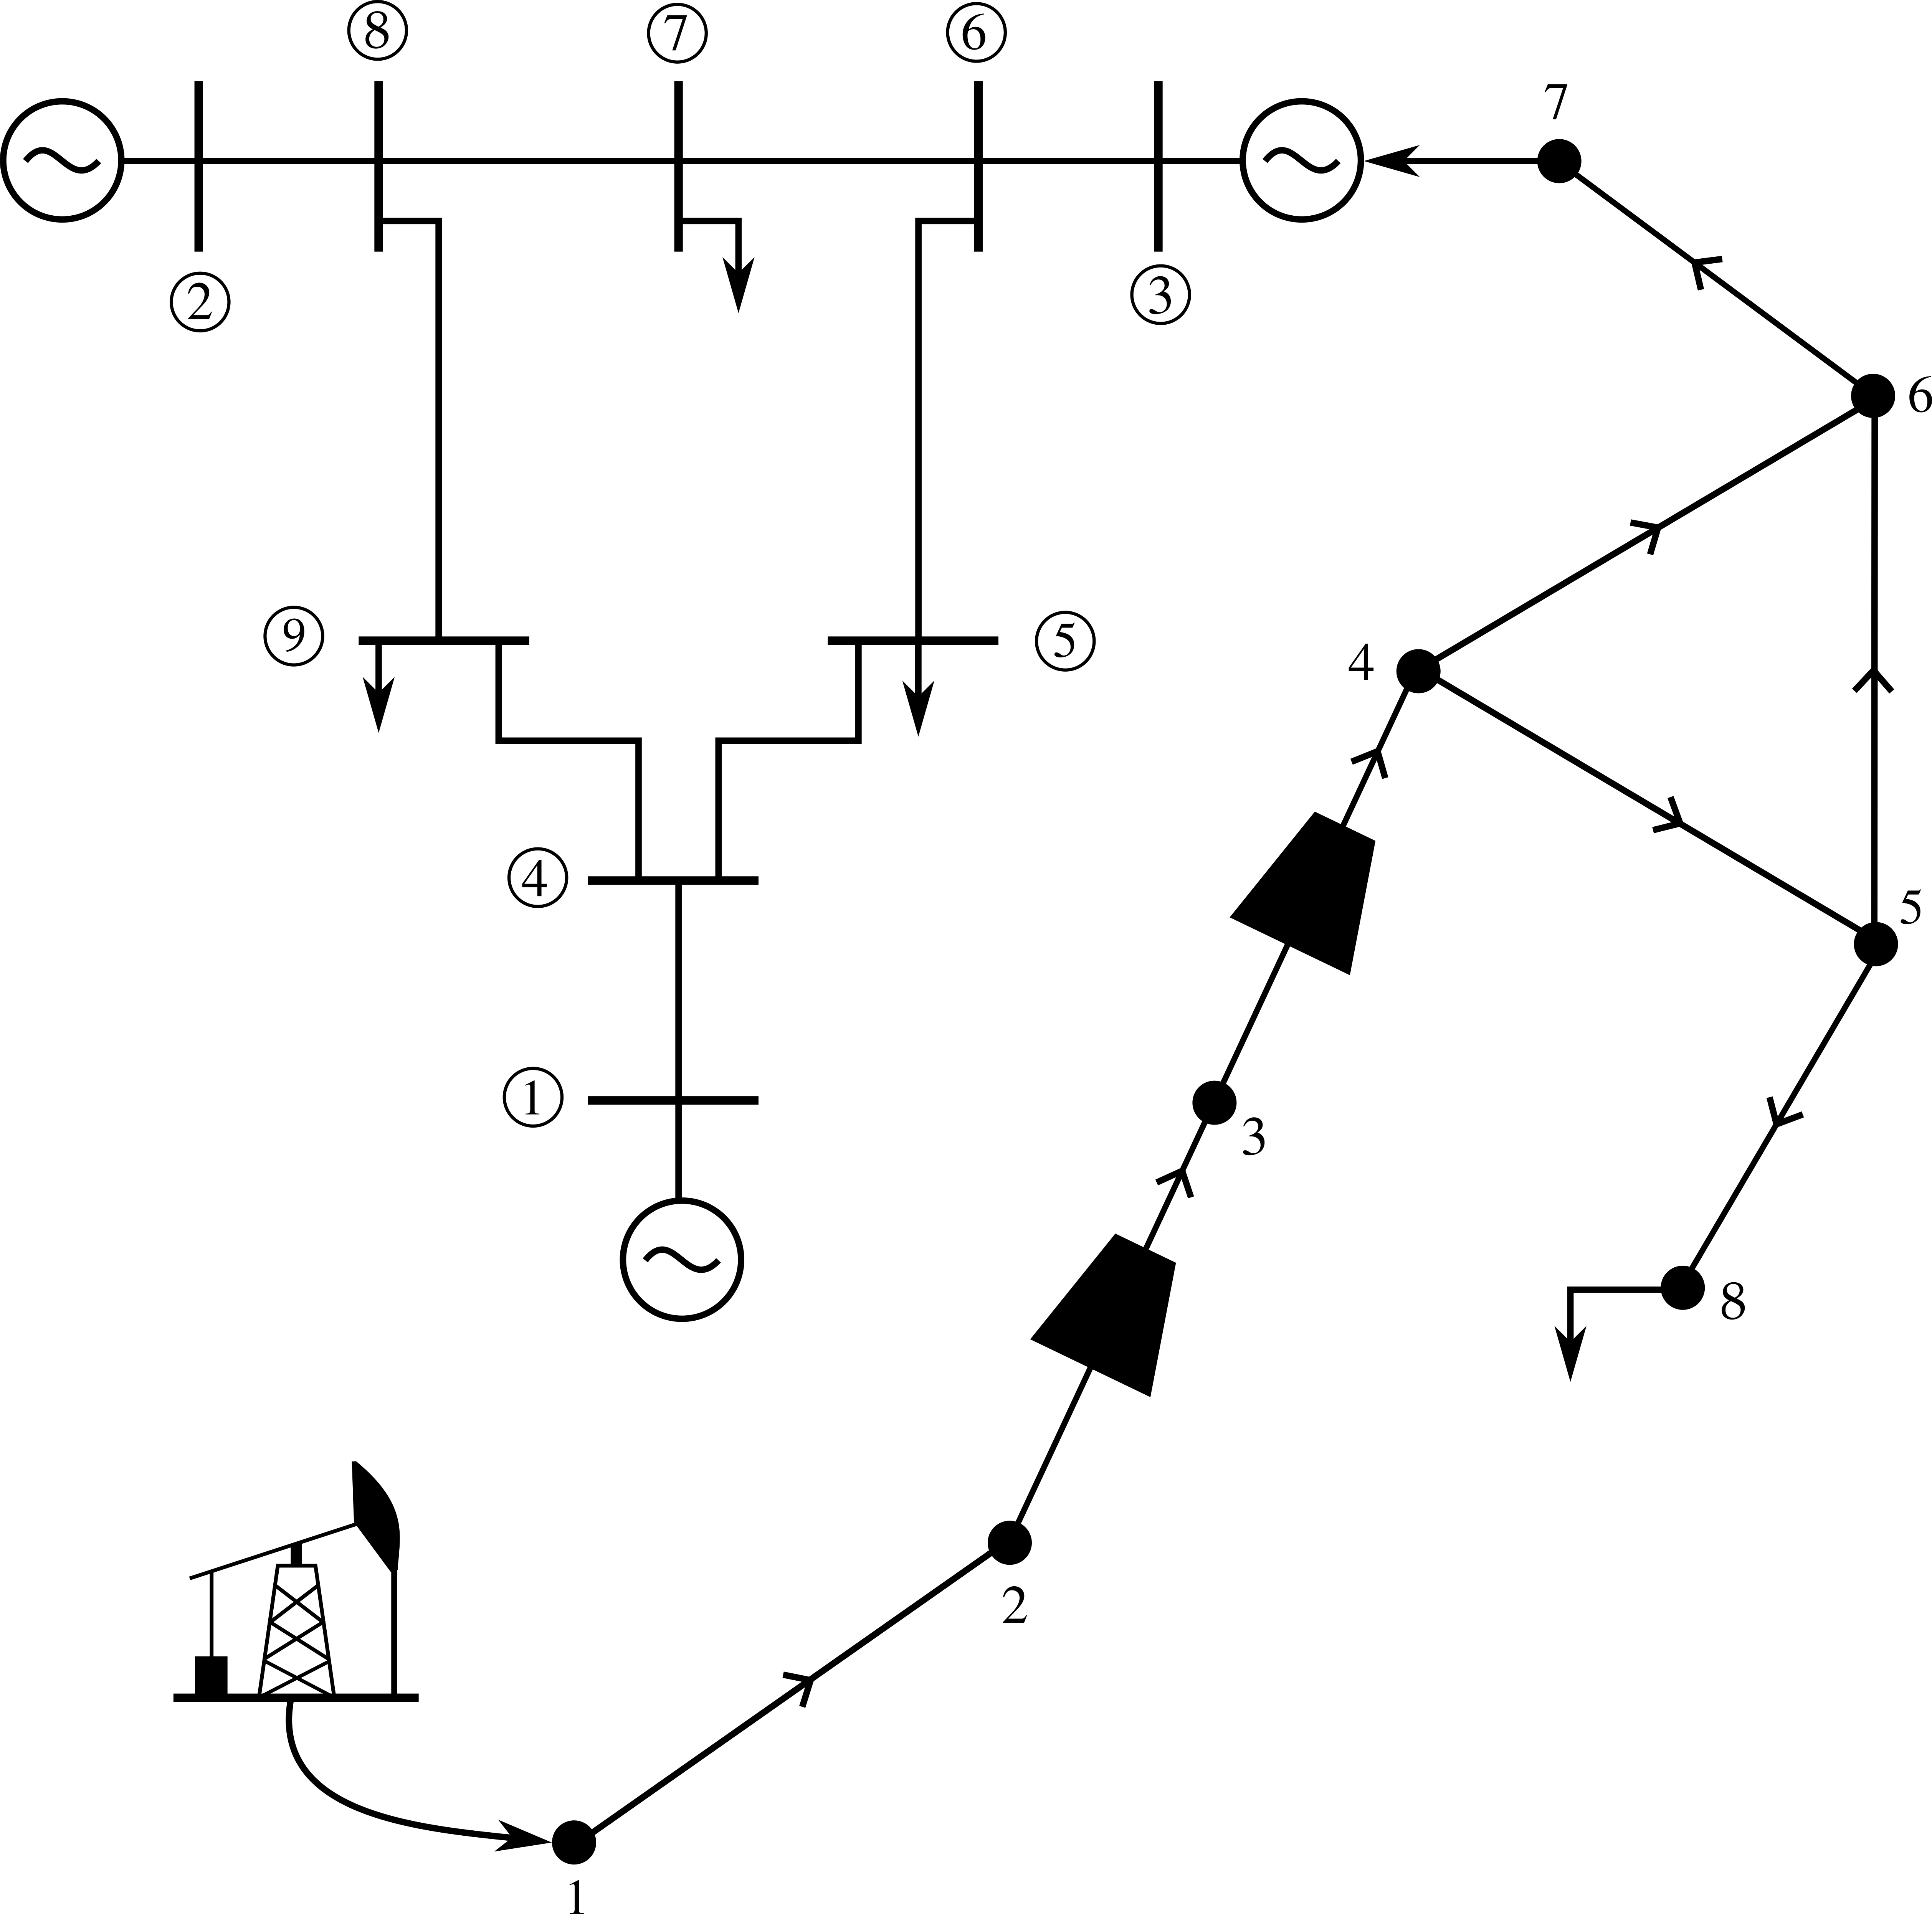
\includegraphics[scale=0.7]{figures/Chapter_MPCC/8 node 9 bus network.png}
    \caption{Integrated system 9/8 used in Case Study I, modified from the MPNG software.~\cite{Wilson_poly}}
    \label{fig:8-9 network}
\end{figure}

To assess the performance of Weymouth approximation approaches on the 9/8 system, a Monte Carlo experiment estimates the cost function and Weymouth error distributions by solving the optimization problem for one day ($\mathcal{T}=\left\lbrace 1\right\rbrace$) one hundred times with uniformly sampled natural gas demands. Further network parameter details can be found in the publicly available repository OptiGasFlow ({\url{https://github.com/cblancom/optigasflow}}, accessed on 05 April 2024). 
 \Cref{fig:blue_test_cost} depicts the cost function histogram for Taylor, SOC, and MPCC approaches. Remarkably, the three histograms evidence identical distribution patterns, leading to regular solutions across approaches.

The boxplots in~\Cref{fig:blue_test_boxplot} show the Weymouth approximation error distribution for each pipeline using three approaches. The error distributions, including median and interquartile range, indicate that MPCC consistently maintains accuracy throughout the network. In contrast, the widely varying errors of the Taylor and SOC approaches suggest a lack of consistency in the achieved solution. Therefore, in a small network, the proposed MPCC approach converges to identical operational costs as Taylor and SOC, even in rationing, while meeting all linear constraints and improving the Weymouth approximation.







